% strongly connected components
\begin{figure}[htb]
\resizebox{\textwidth}{!}{
\subfigure[directed Graph $G$]
{
	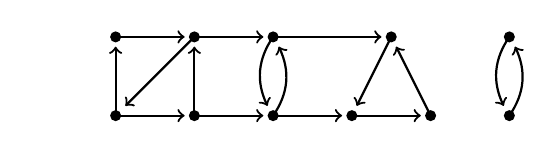
\begin{tikzpicture}
	\node at (0,0) {};
	\node (k1) at (1,0) {};
	\node (k2) at (2,0) {};
	\node (k3) at (2,1) {};
	\node (k4) at (1,1) {};

	\node (k5) at (3,0) {};
	\node (k6) at (3,1) {};

	\node (k7) at (4,0) {};
	\node (k8) at (5,0) {};
	\node (k9) at (4.5,1) {};

	\node (k10) at (6,0) {};
	\node (k11) at (6,1) {};

	\foreach \i in {1,...,11}
	{
		\fill (k\i) circle [radius=2pt];
	};

	\foreach \i / \j in {
	1/2, 2/3, 3/1, 4/3, 1/4,
	7/8, 8/9, 9/7,
	2/5, 3/6,
	5/7,
	6/9}
	{
		\path (k\i.center) edge[->, thick] (k\j);
	};
	\foreach \i / \j in {
	5/6, 6/5,
	10/11, 11/10}
	{
		\path (k\i.center) edge[->, thick, bend right] (k\j);
	};

	\end{tikzpicture}
}
\subfigure[shadow $H$ of Graph $G$]
{
	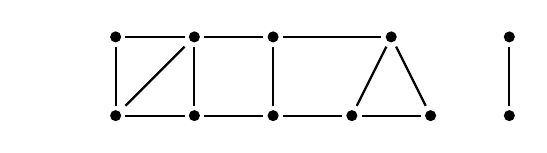
\begin{tikzpicture}
	\node at (0,0) {};
	\node (k1) at (1,0) {};
	\node (k2) at (2,0) {};
	\node (k3) at (2,1) {};
	\node (k4) at (1,1) {};

	\node (k5) at (3,0) {};
	\node (k6) at (3,1) {};

	\node (k7) at (4,0) {};
	\node (k8) at (5,0) {};
	\node (k9) at (4.5,1) {};

	\node (k10) at (6,0) {};
	\node (k11) at (6,1) {};

	\foreach \i in {1,...,11}
	{
		\fill (k\i) circle [radius=2pt];
	};

	\foreach \i / \j in {
	1/2, 2/3, 3/1, 4/3, 1/4,
	7/8, 8/9, 9/7,
	2/5, 3/6,
	5/7,
	6/9,
	5/6, 6/5,
	10/11, 11/10}
	{
		\path (k\i) edge[thick] (k\j);
	};
	\end{tikzpicture}
}}
\resizebox{\textwidth}{!}{
\subfigure[strongly connected components of $G$]
{
	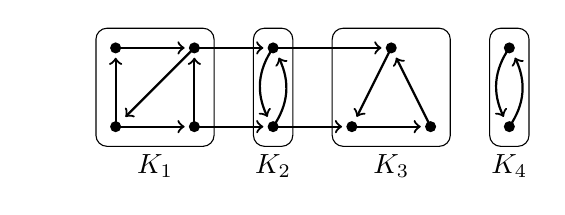
\begin{tikzpicture}
	\node at (0,0) {};
	\node (k1) at (1,0) {};
	\node (k2) at (2,0) {};
	\node (k3) at (2,1) {};
	\node (k4) at (1,1) {};

	\node (k5) at (3,0) {};
	\node (k6) at (3,1) {};

	\node (k7) at (4,0) {};
	\node (k8) at (5,0) {};
	\node (k9) at (4.5,1) {};

	\node (k10) at (6,0) {};
	\node (k11) at (6,1) {};

	\foreach \i in {1,...,11}
	{
		\fill (k\i) circle [radius=2pt];
	};

	\foreach \i / \j in {
	1/2, 2/3, 3/1, 4/3, 1/4,
	7/8, 8/9, 9/7,
	2/5, 3/6,
	5/7,
	6/9}
	{
		\path (k\i.center) edge[->, thick] (k\j);
	};
	\foreach \i / \j in {
	5/6, 6/5,
	10/11, 11/10}
	{
		\path (k\i.center) edge[->, thick, bend right] (k\j);
	};

	\draw[rounded corners] (0.75, -0.25) rectangle (2.25, 1.25);
	\draw[rounded corners] (2.75, -0.25) rectangle (3.25, 1.25);
	\draw[rounded corners] (3.75, -0.25) rectangle (5.25, 1.25);
	\draw[rounded corners] (5.75, -0.25) rectangle (6.25, 1.25);

	\node at (1.5, -0.5) {$K_1$};
	\node at (3.0, -0.5) {$K_2$};
	\node at (4.5, -0.5) {$K_3$};
	\node at (6.0, -0.5) {$K_4$};
	\end{tikzpicture}
}
\subfigure[reduction $G_R$ of Graph $G$]
{
	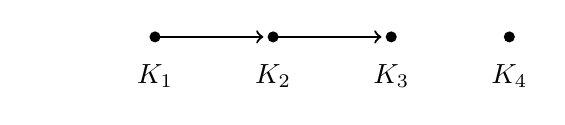
\begin{tikzpicture}
	\node at (0,0) {};
	\node (k1) at (1.5, 0) {};
	\node (k2) at (3.0, 0) {};
	\node (k3) at (4.5, 0) {};
	\node (k4) at (6.0, 0) {};

	\node at (1.5, -0.5) {$K_1$};
	\node at (3.0, -0.5) {$K_2$};
	\node at (4.5, -0.5) {$K_3$};
	\node at (6.0, -0.5) {$K_4$};

	\foreach \i in {1,...,4}
	{
		\fill (k\i) circle [radius=2pt];
	};
	\foreach \i / \j in {1/2, 2/3}
	{
		\path (k\i.center) edge[->, thick] (k\j);
	};
	\end{tikzpicture}
}}
\caption{Graphs}
\end{figure}



